\chapter{Интеллектуальные системы регистрации и анализа проблемных ситуаций, возникающих в ИТ-инфраструктуре предприятия} \label{chapt1}

\section{Сравнительный анализ систем регистрации и устранения проблемных ситуаций} 
В данной Главе рассматриваются имеющиеся на данный момент интеллектуальные системы регистрации и анализа проблемных ситуаций.
\textbf{HP OpenView} \cite{HPOpenView} \cite{HP1} \cite{HP2} \cite{HP3}  является комплексным программным решением по мониторингу ИТ инфраструктуры предприятия. Система имеет множество модулей. Данная система охватывает широкий спектр возможностей:
\begin{itemize}
	\item Мониторинг \cite{HP4} \cite{HP5}
	\item Регистрация инцидентов
	\item Управление системами
\end{itemize}
Система не поддерживает:
\begin{itemize}
	\item Понимание и формализация запросов
	\item Автоматическое исправление проблемы на основе формализации запроса
\end{itemize}


\begin{figure} [h] 
  \center
  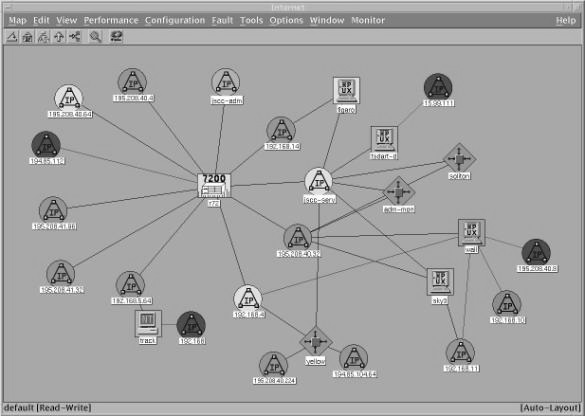
\includegraphics [scale=1.0] {hpopenview}
  \caption{HP OpenView} 
  \label{img:hpopenview}  
\end{figure}

\textbf{ServiceNOW} Средства автоматизации сервиса. Предоставляет следующие возможности:
\begin{itemize}
	\item Регистрация инцидентов
	\item Создание цепи обработки инцидента
\end{itemize}

Система не поддерживает:
\begin{itemize}
	\item Понимание и формализация запросов
	\item Автоматическое исправление проблемы на основе формализации запроса
\end{itemize}

Система широко используется в ИТ инфраструктуре CERN \cite{SN1} \cite{SN2} для регистрации инцидентов и их решения.

\begin{figure} [h] 
  \center
  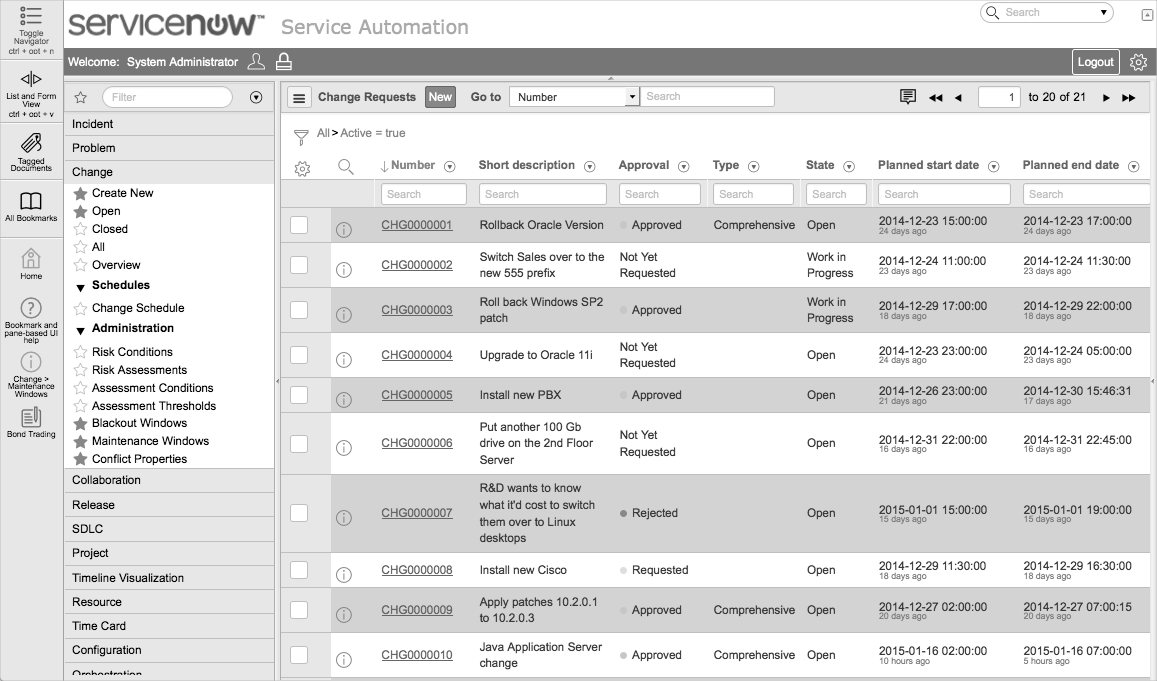
\includegraphics [scale=0.3] {svnow}
  \caption{Service NOW} 
  \label{img:svnow}  
\end{figure}

\textbf{IBMWatson} \ref{img:Watson-Analytics} Вопрос-ответная система поддерживает:
\begin{itemize}
	\item Понимания и формализацию запросов
	\item Поиск решений
\end{itemize}

Система не поддерживает:
\begin{itemize}
	\item Автоматическое исправление проблемы на основе формализации запроса
\end{itemize}
Система широко используется в медицине для постановке диагноза \cite{IBM1} \cite{IBM2} \cite{IBM3} \cite{IBM4}. Система реализует базвые принципы искусственного интеллекта \cite{IBM5} \cite{IBM6}. Разработка велась под супер компьютер IBM Deep Blue \cite{IBM7}.


\begin{figure} [h] 
  \center
  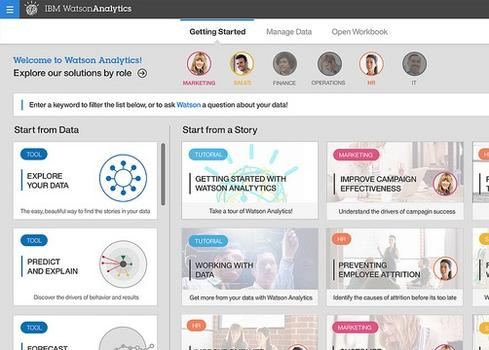
\includegraphics [scale=1.0] {Watson-Analytics}
  \caption{Пример работы системы Watson} 
  \label{img:Watson-Analytics}  
\end{figure}

\textbf{Прочие системы}
Кроме того существуют дополнительные способы автоматизации
\begin{itemize}
	\item Обработка инцидентов посредством регулярных выражений. В таком решение нет гибкости, так как обработка идет путем поиска ключевых слов вне контекста. Метод регулярных выражений частично используется для обработки естественного языка, поиска  \cite{REG1}, диагностики активных систем \cite{REG2}, анализа поведения функций \cite{REG4}, обработки данных в системе eDiscovery \cite{REG5}, в разработке способах программирования \cite{REG3}.
	\item Обработка инцидентов при помощи скриптов. Автоматизирует лишь рутинные операции
\end{itemize}

\section{Определение основных требований к интеллектуальным системам регистрации и анализа проблемных ситуаций в ИТ} \label{sect3_2}

Основными требованиями к системе является следующие:
\begin{itemize}
	\item Мониторинг
	\item Регистрация инцидентов
	\item Управление системами
	\item Создание цепи обработки (Workflow) инцидента
	\item Понимания и формализацию запросов на естественном языке
	\item Поиск решений
	\item Применение решений
	\item Обучение решению инцидента
	\item Умение проводить логические рассуждения: генерализацию, специализацию, синонимичный поиск
\end{itemize}

Требования к системе формировались исходя из возможностей специалистов поддержки, а также анализа проблем, которыми они занимаются. Большинство инцидентов тривиальные и типичные, но все они разные. Для человека проблема "Please insall Firefox" и "Please install Chrome" идентичные, но с точки зрения формализации - нет. Общее в них можно найти взглянув на генерализацию различающейся части. Firefox и Chrome являются пакетами программного обеспечения.



\clearpage

\section{Сравнительный анализ методов и комплексов обработки текстов на естественном языке}


\subsection{Обработка эталонных текстов} \label{sect2_1}
В данном разделе проводится обзор обработчиков естественного языка. За основу были взяты инциденты из выгрузки систем поддержки ОАО "ICL КПО-ВС". \\
Ввиду специфики области основным языком был выбран английский язык. Был сформирован список из типичных эталонных фраз, на которых тестировались обработчики естественного языка. Фразы были выявлены путем анализа существующих отчетов об инцидентах. Примерами инцидентов являются следующие инциденты:\\
\textbf{Инцидент 1}
\textit{
User had received wrong application. User has ordered Wordfinder Business Economical for her service tag 7Q4TC3J, there is completed order in LOT with number ITCOORD-18125. However she received wrong version, she received Wordfinder Tehcnical instead of Business Economical. Please assist.
}\\
\textbf{Инцидент 2}
\textit{
Laptop – user has almost full C:\ but when he looks in the properties of the files and folders on C:\ they are only 40GB and he has a 55GB drive.
}\\
\textbf{Инцидент 3}
\textit{
User cannot find Produkt Manageron start menu. Please reinstall. 
}\\
\textbf{Инцидент 4}
\textit{
User needs to have pdf 995 re-installed please.
}\\

Во время анализа были использованы следующие обработчики естественного языка:
\begin {enumerate}
	\item{Open NLP}\cite{OpenNLP}
	\item{RelEx}\cite{OpenCogRelex}
	\item{StanfordParser}\cite{StanfordParser}
\end {enumerate}

Результат работы вычислялся при помощи метрик, представленных в Таблице\ref{Metrics}. 

\begin{table} [htbp]
  \centering
  \parbox{15cm}{\caption{Таблица метрик}\label{Metrics}}
%  \begin{center}
  \begin{tabular}{| p{5cm} ||p{5cm}|| p{5cm} |}
  \hline
  \hline
Метрика & Описание & Формула \\
  \hline
  \hline
Аккуратность	& Понимание текста обработчиком & 
$$ 
Ac=\frac{1-x}{y}
$$ где x- количество нераспознанныx слов, y количество распознанных \\
 \hline
Успешно обработанные	& Успешно обработанные инциденты & 
$$ 
P=\frac{x}{100}
$$ где x успешно обработанные \\
 \hline
Не успешно обработанные	& Неуспешно обработанные инциденты & 
$$ 
N=\frac{y}{100}
$$ где y неуспешные инциденты \\
 \hline
Результативность	& Общая результативность обработчика & 
$$ 
R=\frac{P}{N}
$$  \\
  \hline
  Общий бал	& Общая оценка обработчика & 
$$ 
T=Ac+R
$$  \\
  \hline
  \hline
  \end{tabular}
%  \end{center}
\end{table}

Результаты приведены на сводной диаграмме Рисунок \ref{img:ParserComp}

\begin{figure} [h] 
  \center
  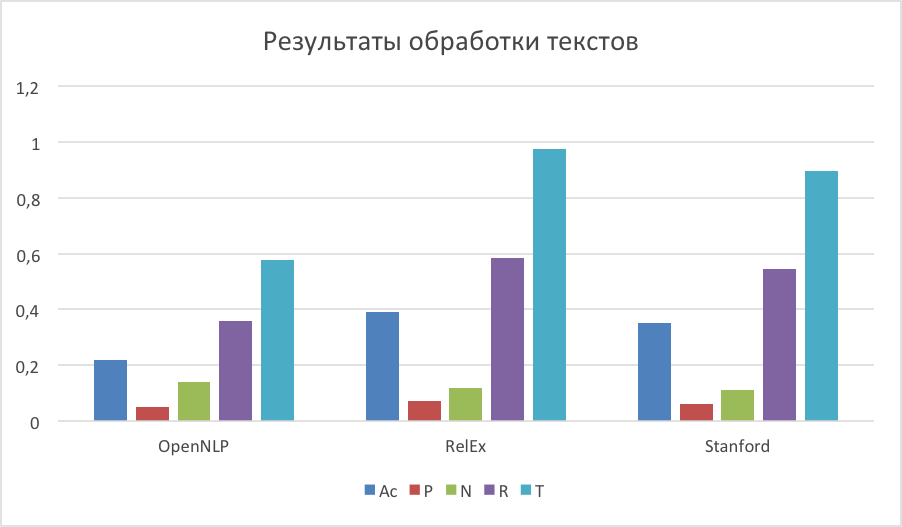
\includegraphics [scale=1.0] {ParserCompare}
  \caption{Результаты обработки текстов} 
  \label{img:ParserComp}  
\end{figure}

Из диаграммы видно, что наилучшее результаты показывает обработчик RelEx\cite{OpenCogRelex}. После анализа необработанных инцидентов было выявлено нескольких проблем у всех обработчиков:
\begin{enumerate}
	\item Невозможности корректировки простых грамматических ошибок, связанных с пропущенными пробелами или неверным форматированием. Ошибки первого типа.
	\item Ошибки неверной интерпретации слов в предложении. Например, слово please интерпретировалось как глагол, хотя является по смыслу «формой вежливости». Ошибки второго типа.
\end{enumerate}	

	
 
\clearpage
\subsection{Обработка текстов с ошибками} \label{sect2_2}

По результатам прошлого раздела было решено выбрать в качестве обработчика естественного языка RelEx, но были выявлены некоторые проблемы. Было принято решение исправить данные проблемы при помощи предварительной обработки текста. Предварительная обработка текста была разбита на несколько фаз:
\begin{enumerate}
	\item Комплексная корректировка ошибок
	\item Обработка при помощи внутренней базы знаний
\end{enumerate}
Для того, чтобы избавится от орфографический, синтаксических ошибок используется составной корректировщик. Данный компонент имеет модульную структуру и применяет корректировку последовательно.
\begin{figure} [h] 
  \center
  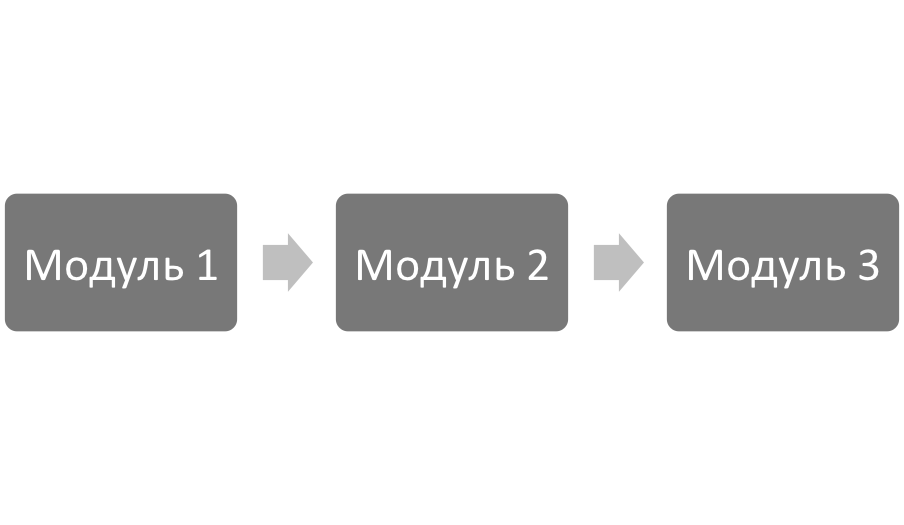
\includegraphics [scale=1.0] {SpellCorrector}
  \caption{Архитектура предварительной обработки текста} 
  \label{img:SpellCorrector}  
\end{figure}

Для данного компонента были написаны модули корректировки:
\begin{itemize}
	\item Google API
	\item After The Deadline
\end{itemize}
Таким образом удалось исправить большинство ошибок, связанный с синтаксисом, грамматикой, орфографией. Также удалось исправить ошибки неверного написания: лишних пробелов, пропущенных запятых, пропущенных точек.
По-прежнему остается проблема обработки неверной интерпретации слов в тексте. \\

Для корректировка ошибок второго типа был использована инъекция в работу парсера RelEx. Вввиду OpenSource природы проекта, модульности был подменен модуль извлечения и обработки слов в предложения. Стандартный процесс обработки был разбит на «предобработку» и «обработку». Стадия «обработки» включала в себя алгоритм работы такой же как был до этого в модули, на стадии «предобработки» управление передается модулю основному приложению, который проверяет данное слово на предмет его вхождения во внутреннюю Базу Знаний и если таковое имеется, то приложение передает соответствующие корректировки в модуль

\clearpage
\subsection{Сравнение средств обработки русского и английского языков} \label{sect2_3}
Средства обработки естественного языка принято относить в большому классу средств NLP – Natural Language Processing. Для английского языка существует множество открытых средств обработки естественного языка, для русского языка найти их гораздо сложнее. Рассмотрим архитектуру средств обработки естественного языка на примере OpenCog RelEx. \\
OpenCog RelEx использует результаты обработки Link Grammar \cite{linkgrammar}. Link Grammar поддерживает множество языков: английский, русский, турецкий, немецкий и т.д.  RelEx использует вывод LG и преобразует его в формат связей.
\textbf{Пример 1}. User is unable to start KDP web, please reinstall Java.\\
\textbf{Результат} 
\begin{verbatim}
		_obj(start, KBP)
pos(start, verb)
inflection-TAG(start, .v)
tense(start, present)
pos([web], WORD)
noun_number(KBP, singular)
definite-FLAG(KBP, T)
pos(KBP, noun)
_advmod(reinstall, please)
pos(reinstall, verb)
inflection-TAG(reinstall, .v)
tense(reinstall, present)
pos(please, adv)
inflection-TAG(please, .e)
noun_number(Java, singular)
definite-FLAG(Java, T)
pos(Java, noun)
pos(., punctuation)
_obj(,, Java)
pos(,, verb)
tense(,, infinitive)
HYP(,, T)
_to-do(unable, ,)
pos(unable, adj)
inflection-TAG(unable, .a)
tense(unable, present)
pos(to, prep)
inflection-TAG(to, .r)
pos(be, verb)
inflection-TAG(be, .v)
_predadj(User, unable)
noun_number(User, singular)
definite-FLAG(User, T)
pos(User, noun)

\end{verbatim}



Возьмем разбор слова start. В результате мы получаем несколько отношений:
\begin{itemize}
	\item pos(start, verb) - start глагол
	\item tense(start, present) - время настоящее
	\item inflection-TAG(start, .v) -  метод обозначения на схеме (индекс)
\end{itemize}

На их основе можно формализовать приложение на естественном языке. Остальные парсера пока не поддерживают русский язык. Существуют открытые проекты, но они еще недостаточно развиты.
\section{Выводы}
В данной главе были рассмотрены существующие на данный момент системы в области обработки экспертной информации в области обслуживания программного обеспечения и информационной архитектуры.
Все рассмотренные системы не соответствуют полному комплексу необходимых требований. В Таблице \ref{Comparsion} приведены сводные данные по системам. В главе также выработаны критерии сравнения обработчиков естественного языка и выполнен основной анализ обработчиков естественного языка. Ввиду развитости и доступности было решено использовать OpenCog RelEx.

\begin{longtable}{|p{6cm}|p{0.5cm}|p{0.5cm}|p{0.5cm}|}
 \caption[Сравнительный анализ существующих решений]{Сравнительный анализ существующих решений}\label{Comparsion} \\ 
 \hline
 
 \multicolumn{1}{|c|}{\textbf{Сравнительный пункт}} & \multicolumn{1}{c|}{\textbf{HP Open View}} & \multicolumn{1}{c|}{\textbf{ServiceNOW}} & \multicolumn{1}{c|}{\textbf{IBM Watson}} \\ \hline 
\endfirsthead
\multicolumn{2}{c}%
{{\bfseries \tablename\ \thetable{} -- продолжение}} \\
\hline \multicolumn{1}{|c|}{\textbf{Сравнительный пункт}} & \multicolumn{1}{c|}{\textbf{HP Open View}} & \multicolumn{1}{c|}{\textbf{ServiceNOW}} & \multicolumn{1}{c|}{\textbf{IBM Watson}}  \\ \hline 
\endhead

\hline \multicolumn{2}{|r|}{{Продолжение следует}} \\ \hline
\endfoot

\hline \hline
\endlastfoot
\hline
   Мониторинг & Да & Да & Да \\
   \hline
   Регистрация инцидентов & Да & Да & Да\\
   \hline
   Управление системами & Да & Нет & Нет \\
   \hline 
   Создание цепи обработки (Workflow) инцидента & Да & Да & Нет \\
   \hline 
   Понимания и формализацию запросов на естественном языке & Нет & Нет & Да \\
   \hline 
   Поиск решений & Нет & Нет & Да \\
   \hline 
   Применение решений & Нет & Нет & Нет \\
   \hline
   Обучение решению инцидента & Нет & Нет & Да \\
   \hline
   Умение проводить логические рассуждения: генерализацию, специализацию, синонимичный поиск & Нет & Нет & Нет \\
   \hline
   \textbf{Итоговые очки} & 4 & 3 & 5 \\
   \hline 
\end{longtable}
\clearpage
